%% Master Thesis Template
%% Please update the specification through this link: https://daim.idi.ntnu.no/howto_thesis_submission.pdf

\documentclass[pdftex,10pt,b5paper,twoside]{book}
\usepackage[lmargin=25mm,rmargin=25mm,tmargin=27mm,bmargin=30mm]{geometry}

\usepackage{setspace}
\usepackage{graphicx}
\usepackage{amssymb}
\usepackage{mathrsfs}
\usepackage{amsthm}
\usepackage{amsmath}

\usepackage{color}
\usepackage[Lenny]{fncychap}
\usepackage[pdftex,bookmarks=true]{hyperref}
\usepackage[pdftex]{hyperref}
\hypersetup{
    colorlinks,%
    citecolor=black,%
    filecolor=black,%
    linkcolor=black,%
    urlcolor=black
}
\usepackage[font=small,labelfont=bf]{caption}
\usepackage{fancyhdr}
\usepackage{times}
%\usepackage[intoc]{nomencl}
%\renewcommand{\nomname}{List of Abbreviations}
%\makenomenclature
\usepackage{natbib}
\usepackage{float}
%\floatstyle{boxed} 
\restylefloat{figure}

\usepackage{algorithm} 
\usepackage{algpseudocode} 

% ShareLaTeX does not support glossaries now. Sorry...
%\usepackage[number=none]{glossary}
%\makeglossary
%\newglossarytype[abr]{abbr}{abt}{abl}
%\newglossarytype[alg]{acronyms}{acr}{acn}
%\newcommand{\abbrname}{Abbreviations} 
%\newcommand{\shortabbrname}{Abbreviations}
%%\makeabbr
\newcommand{\HRule}{\rule{\linewidth}{0.5mm}}

\renewcommand*\contentsname{Table of Contents}

\pagestyle{fancy}
\fancyhf{}
\renewcommand{\chaptermark}[1]{\markboth{\chaptername\ \thechapter.\ #1}{}}
\renewcommand{\sectionmark}[1]{\markright{\thesection\ #1}}
\renewcommand{\headrulewidth}{0.1ex}
\renewcommand{\footrulewidth}{0.1ex}
\fancypagestyle{plain}{\fancyhf{}\fancyfoot[LE,RO]{\thepage}\renewcommand{\headrulewidth}{0ex}}

\begin{document}
\graphicspath{{fig/}}

%% PART 1
%%The title page will be automatically generated and added by the DAIM system

%This is the Titlepage
%%=========================================
%This is the Titlepage
%%=========================================
\thispagestyle{empty}

%\mbox{}\\[3pc]
%\hrulefill
\begin{center}

\Large{NTNU}\\
\normalsize{Norwegian University of Science and Technology}\\
[3pc]
\Large{TMA4500 - Specialization Project}\\

\Huge{\hrulefill\\Modelling time varying synaptic weights from spike train data \\\hrulefill}\\[2pc]
%Ultra-Low Power Motion Sensors for High Volume IoT Applications 
\small{Author:}\\\Large{Astrid Langsrud}\\
\mbox{}\\[3pc]
\large{January 2020}\\[2pc]

\small{Supervisor: Benjamin Dunn}\\
\small{Co-supervisor: Claudia Battistin}

\end{center}
\vfill

\begin{figure}[h]
\centering

\includegraphics[scale=0.5]{fig/ntnu-logo.jpg}
\label{fig:frontpage_logo}
\end{figure}

%% Optional

%% PART 2
\clearpage
\pagenumbering{roman} 				
\setcounter{page}{1}

\pagestyle{fancy}
\fancyhf{}
\renewcommand{\chaptermark}[1]{\markboth{\chaptername\ \thechapter.\ #1}{}}
\renewcommand{\sectionmark}[1]{\markright{\thesection\ #1}}
\renewcommand{\headrulewidth}{0.1ex}
\renewcommand{\footrulewidth}{0.1ex}
\fancyfoot[LE,RO]{\thepage}
\fancypagestyle{plain}{\fancyhf{}\fancyfoot[LE,RO]{\thepage}\renewcommand{\headrulewidth}{0ex}}

\section*{\Huge Summary}
\addcontentsline{toc}{chapter}{Summary}	
$\\[0.5cm]$



\clearpage		%% Optional
#\section*{\Huge Preface}
\addcontentsline{toc}{chapter}{Preface}
$\\[0.5cm]$

\noindent Write your preface here...

\cleardoublepage		%% Optional
\tableofcontents
\addcontentsline{toc}{chapter}{Table of Contents}
\clearpage


\pagenumbering{arabic}

%% PART 3 -- The Chapters
%===================================== CHAP 1 =================================

\chapter{Introduction}

%\begin{itemize}
    %\item Begin with something short about what I am going to write about, to set the cotext
    %\item Rewrite the introduction in the end, so I can refer to my conclusions ect...
    %\item Be clear on specifying the aim of this thesis
%\end{itemize}


%Alzheimer's disease is a very common form of dementia, and one of the most "common causes of death for older people" (https://www.nia.nih.gov/health/alzheimers-disease-fact-sheet). According to World Alzheimers report 2018, 50 million people suffer from dementia worldwide, and about two thirds of them have Alzheimers. This is a disease that is highly related to age, so as people live longer, Alzheimers become a more common disease. By 2050 the number of Alzheimers patients is expected to triple.

%Alzheimer's disease is a neurodegenerative disease that slowly develops over many years. On average, a person lives for seven years after the diagnose is set. One of the typical first symptoms is struggling with episodic memory. As the disease proceeds the patient will get personality changes and language troubles, and eventually the body functions will collapse and the patient will die.The suffering is big for the patients and their family.  Also the global cost for the disease is massive. The money spent on dementia was estimated to be 1 trillion US dollars for 2018 ( Alzheimers report 2018).
%Today there are no good treatments of the disease, and what causes it and how it develops in the brains is not completely understood.  By its severe consequences for individuals and for the society, it is no doubt that research on this disease is of importance.

%Because of its major impacts, Alzheimer's disease is a popular field to do research on. At the Kavli institute at NTNU they have an ongoing project where they record neural activity in brains from rats with and without Alzheimers. For my master thesis in the spring 2020 I will get access to the data from these experiments, and apply statistical analysis. 

%The data takes the form of time points for spiking of # individual neurons over time. It is known that neurons connect to each other, so that the activity of one neuron can affect the activity of another. When scientist model a neural network, these connections are typically regarded as being fixed. However, in reality the brain is a dynamic system. The changing of neural connections in the brain is referred to as synaptic plasticity, and gives rise to learning and memory. Since the main  characteristics of Alzheimer's disease is troubling with memory and learning, an hypothesis is that the the synaptic plasticity in Alzheimers brains has some differences to that in normal brains. So the goal for my master thesis develop a model for the dynamics of the neural connections, and investigate if there is a significant difference between data recorded from networks with Alzheimer's compared to those without. 

%This project report is a prework for the master thesis. The aim of this project is to develop a model for inferring synaptic plasticity, and perform various simple test cases with simulated data to explore the functionality and limitations of the model. The statistical framework in this thesis is inspired by a paper from Harvard University, "A framework for studying synaptic plasticity with neural spike train data", \cite{Linderman}. The paper describes a way of using GLM and particle Markov Chain Monte Carlo for modeling synaptic plasticity. The way in which the synaptic connections are changing seems to follow some rules, called "learning rules". In the paper two kinds of learning rules are presented and compared. ... Something more


A living brain is a dynamical system where connections between neurons can strengthen and weaken over time. This phenomenon, known as \textit{synaptic plasticity}, has shown to follow some underlying patterns. It is an essential mechanism for learning and memory, and it is therefore believed that these patterns might be affected by memory related diseases, such as Alzheimer's. The focus in this project is to develop a method for studying synaptic plasticity, with the idea that it could be used to search for differences between brains with and without Alzheimer's, when appropriate neural activity data is available.  \\

Alzheimer's disease is a common form of dementia, and is a typical cause of death for older people. According to World Alzheimers report 2018, 50 million people suffer from dementia worldwide, and about two thirds of them have Alzheimers. This is a disease that is highly related to age, so as people live longer, Alzheimer’s will become even more common. The cost of the disease for the society, as well as for the patients, is therefore massive and growing.

Because of its major impacts, Alzheimer's disease is a popular field to do research on. At the Kavli institute at NTNU they have an ongoing project to record neural activity in brains from rats with and without Alzheimer’s. This work will build on the intention to be applied to these recordings.

%Therefore, a description of the relevant properties from neuroscience and from these lab experiments is included.

The main goal of this specialization project is to develop a method for learning time-varying connections between neurons and perform various simple test cases with simulated data to explore its functionality and limitations. The statistical framework in this thesis is inspired by a paper from Harvard University, "A framework for studying synaptic plasticity with neural spike train data", \cite{Linderman}. Also, this work will set the basis for my master thesis, in which the method developed here will be extended to infer synaptic plasticity rules and potentially employed to compare Alzheimer's brains with healthy ones.

The relevant context from neuroscience, as well as a description of the background for the data is provided in chapter \ref{ch:2}. The system will be modelled with a Bernoulli Generalized Linear Model following underlying specified learning rules. To make inference it will be taken a Bayesian approach, and a MCMC algorithm will be used. The necessary theory and background for this is given in chapter \ref{ch:theory}. Neural spike activity will be simulated, and test cases for making inference on the synaptic connection will be implemented. The method for these is described in chapter \ref{ch:methods} and the corresponding results will be presented in chapter \ref{ch:results}.


%Relevant background from neurosience is described in chapter \ref{ch:2}. \ref{ch:theory} \ref{ch:methods} \ref{ch:results} \ref{ch:6}		%% Edit each chapter
%===================================== CHAP 2 =================================

\chapter{Neuroscience context}
\label{ch:2}

Before going into the statistics and modeling, it is useful to present some context for the work. The aim of this chapter is to describe the relevant concepts from neuroscience, explain the background for the data material and provide a practical understanding. Section \ref{NandC} gives a brief description of signaling and connectivity in neural networks; the source used for this section is the book \textit{Neuroscience}, by Purves. The hallmarks for Alzheimer's disease in the brain are described in section \ref{EandA}, whose content is based on \cite{Gomez} and \cite{Witter:2011}. Section \ref{Lab} provides an outline of the lab experiments where the data that is background for this project comes from. As mentioned in the introduction, only simulated data will be used for analysis in this project. However, the methods are developed with the ultimate goal of analyzing the real data described here, which will be the object of the master project. 

\section{Concepts from neuroscience}

\subsection{Neuron and connections}\\
\label{NandC}

The basic computational unit in the brain is the nerve cell. It consists of a cell body (soma), an axon and dendrites, as illustrated in figure \ref{neuron}.
\begin{figure}[h]
    \caption{Illustration of a neuron.}
    \label{neuron}
    \centering
    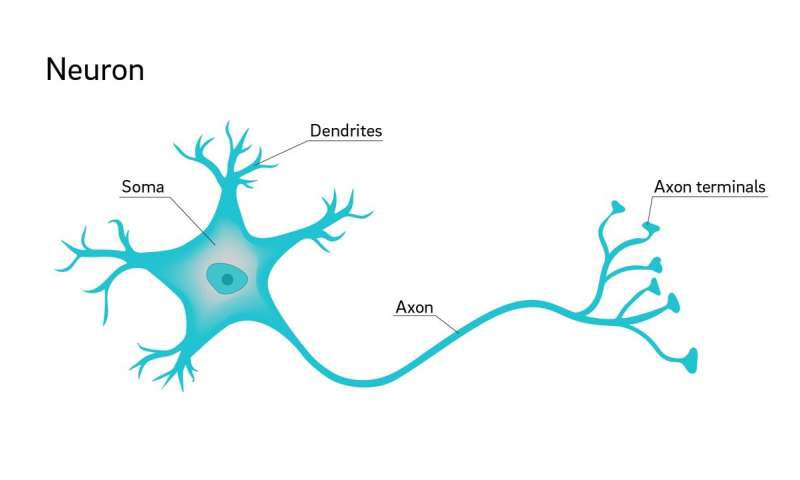
\includegraphics[scale=0.3]{Neuron.jpeg}
\end{figure} 

The computational ability of a neuron relies on its electrochemical properties. When a neuron is at rest, there is a constant potential difference across the inside and the outside of its cell membrane. This is known as the \textit{resting potential}. Ion channels embedded in the membrane allow ions to flow in and out, which can disturb the potential difference away from this equilibrium. If the voltage hits a certain threshold value, a rapid depolarization will be initiated. This phenomenon is known as an \textit{action potential}, also referred to as neuron \textit{firing} or \textit{spiking}. Whenever the threshold potential is reached, the action potential will take place no matter what. In other words there is an all-or-non property, in its typical wave form (see figure \ref{AP}). After being initiated in the soma the action potential will propagate along the axon, as illustrated to the right of figure \ref{AP}.

\begin{figure}[h]
\caption{Graphical representation of an action potential (left). Illustration of action potential propagating along axon (right).}
\label{AP}
\begin{subfigure}
\centering
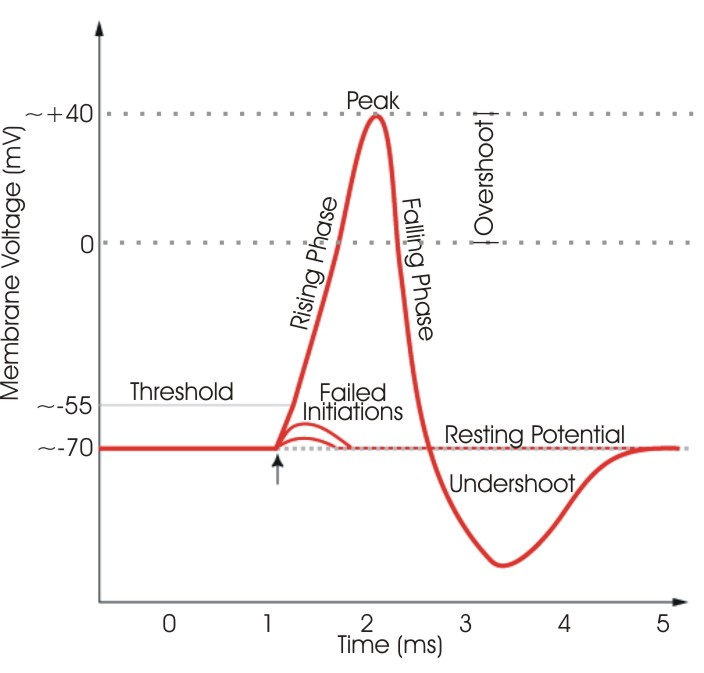
\includegraphics[scale=0.7]{AP.jpg}
\end{subfigure}
\begin{subfigure}
\centering
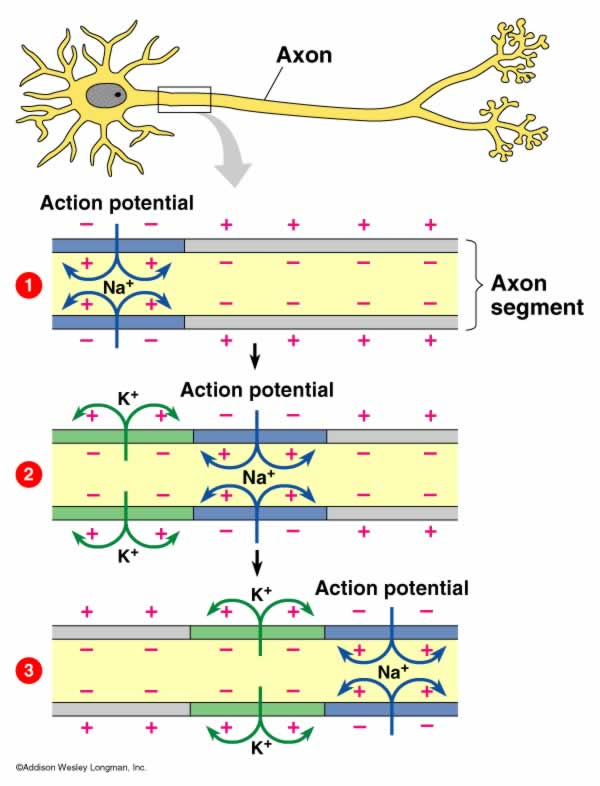
\includegraphics[scale=0.21]{Axjk4.jpg}
\end{subfigure}
\end{figure} 

The voltage increase that eventually leads to an action potential typically happens in response to stimuli from other neurons. Neurons in the brain are indeed connected to each other in a complex network. These connections are between an axon of one neuron and a dendrite of another, and are referred to as \textit{synapses}. A synapse is in practice a short gap where chemical units, called neurotransmitters, are allowed to flow from the axon of a \textit{presynaptic} neuron to the dendrite of a \textit{postsynaptic} neuron. This neurotransmitter flow, the signal, happens when the presynaptic neuron undergoes an action potential and causes an alteration in the probability with which post-synaptic ion channels open and close. This input from the pre-synaptic neuron contributes to the membrane potential (together with on average $10^4$ other neurons in the mammalian brain) which  may develop into an action potential if the threshold is reached. Sometimes the electrical signal from the presynaptic neuron increases the likelihood of an action potential to also arise in the postsynaptic neuron. In this case we say that the synapse is excitatory. This property gives rise to the possibility for a signal to propagate through the neural network, and eventually end up for example in a muscle and cause a contraction. There are also synapses that decrease the chance that the postsynaptic neuron will fire when activated. These are called inhibitory synapses.

The strength of these neural connections is not fixed, but can change over time. Strength in this sense refers to the probability that the spiking in the postsynaptic neuron will be affected by an action potential in the presynaptic neuron. A frequent activation of a synapse can strengthen the synaptic connection over time. This phenomenon is called \textit{long-term potentiation} (LTP) of a synapse. Other times activation of a synapse can weaken the connection over time. This is called \textit{long-term depression} (LTD). These changes of connections are referred to as synaptic plasticity, which is one of the basic mechanisms underlying learning and memory. \\

\subsection{Alzheimer's disease and the entorhinal cortex}
\label{EandA}

If a patient has struggles from Alzheimer's disease, the brain will eventually shrink significantly. This is due to loss of synapses and neurons, which is one of the main characteristic of the disease. Figure \ref{EC} (right) illustrates how a brain can look like after having AD for many years. Exactly what causes these losses is still not known, but it is assumed that the accumulation of some protein types called amyloid plaques and neurofirbillary tangles are involved. Another hallmark of AD is impaired neural activity, which may be related to dysfunctional plasticity mechanisms (\cite{Zott}). Therefore, it is interesting to investigate whether healthy brains and brains with AD can be distinguished due to their synaptic plasticity properties.

\begin{figure}[h]
    \caption{(Left) Illustration of brain showing location of the Entorhinal cortex. (Right) Visual comparison of healthy brain and brain with Alzheimer's disease.}
    \label{EC}
    \centering
    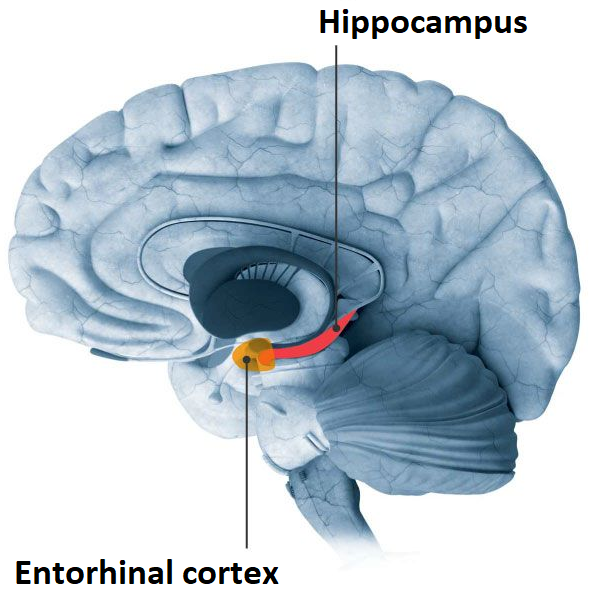
\includegraphics[scale=0.35]{Entorhinal_cortex2.png}
    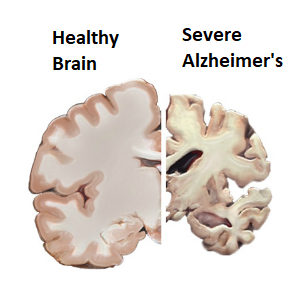
\includegraphics[scale=0.8]{fig/Alzheimers_picture.png}    
    \label{brain}
\end{figure} 

One target area in the brain for Alzheimer's research is the \textit{entorhinal cortex}, which is associated with the earliest indications of AD. The entorhinal cortex is a brain region that is phylogenetically conserved across species, so research on how AD develops in rat's entorhinal cortex can give insights for humans as well. It is found in the medial temporal lobe and functions as a gateway between the neocortex and the hippocampus, which is known to be involved in declarative memory and learning. The position  of the entorhinal cortex in the brain is shown in figure \ref{EC} (left). The entorhinal cortex is commonly subdivided into six layers, I-VI. Cells in layer II of the entorhinal cortex are shown to be affected in the initial stages of AD. Therefore layer II neurons are object of the experiments we will get the data from to study how AD affects the synaptic plasticity.




\section{Data material}

\label{Lab}\\
The data material that is the background for this project is electric potential recordings from in-vitro cultured neural networks from rat brains. Rats do not get Alzheimer's naturally, so AD rats are designed with a genetic mutation that gives rise to amyloid plaque accumulation in their brains. It was shown that at an age of 8 months, mice with this mutation have learning impairments and behavioural differences from healthy mice (\cite{Radde}). 

In short, tissue from layer II of the entorhinal cortex is gathered by microdissection from rat brains (\cite{Katrine}), and the embedded neurons are dissociated from their biological substrate to be plated into a dish. Next the seeded neurons are cultured in a mean, which allows them to survive and grow new connections. Once the network is mature, microelectrode arrays, a sheet of equally spaced needle electrodes, are then used to record the electrical activity of the neurons. Preferably each electrode should measure the activity of one neuron only. However, the recordings are extracellular, which means that the electrodes might pick up signals from several neurons. Therefore, a spike sorting procedure is performed to assign the recorded action potentials to single neurons. 

It is the time points for the action potentials that are of interest, and not the actual voltage values. Hence, the relevant data material is a sequence of recorded time points for the action potentials for each neuron, in the time interval $[0,K]$. This can be written as, 
\begin{equation}
\label{eq:AP}
    \{\{a_i\}\}_{i=1}^{N} = \{a_{i1}, a_{i2}, ...\}_{i=1}^{N} \quad a_{ix} \in [0,K]
\end{equation}

where $a_{ix}$ is the recorded time for the $x'th$ action potential of neuron $i$, $a_{ix-1} < a_{ix}$, and $i=1,2,...,N$ labels the neurons. Such a sequence of time stamps for a single firing neuron is called a \textit{spike train}.\\



%One electrode can measure the electrical activity of one neuron over time interval $[0,K]$. When a neuron undergoes an action potential, this will appear as a peak in these recordings.



\cleardoublepage
%===================================== CHAP 3 =================================

\chapter{Background and theory}
\label{ch:theory}

The goal is to characterize the dynamics of synaptic connections based on the data material from the lab experiments. Since we know that simultaneous spiking of the presynaptic and postsynaptic neuron affects the synaptic connection, it is relevant to study the changing of neuronal spike rates in relation to the spiking of the surrounding neurons. For one neuron at one time step, the situation of spiking or not spiking can be considered as a Bernoulli process, with some time dependent spiking rate $\lambda (t)$. This spiking rate can be expressed function of the spike history of the neuron itself and of the other neurons, which can be modelled using a Generalized Linear Model (GLM). The relevant statistical theory is described in section \ref{sec:stats}. Section \ref{Intro_GLM} provides a general introduction to the GLM framework and presents how it looks like for a Bernoulli distribution. In section \ref{sec:Inference} it is explained how inference in GLMs can be made according to the maximum likelihood and gradient based methods. 

Gradient based methods with maximum likelihood works well if the problem is convex and enough information is stored in the data. If we have a system with stationary connectivity, this approach is suitable. However, for a network of N neurons with dynamical connections over T time steps, the number of parameters is of $O(N^2 \times T)$, whereas the number of data points is of $O(N \times T)$. This means that the system with dynamical connections is undersampled for the technique presented in section \ref{sec:Inference}. However, there are big correlations in time, and we have hypotheses on the connectivity dynamics from the learning rules. Therefore, taking advantage of the prior knowledge with a Bayesian approach is a natural choice. A description of the Bayesian framework is given in section \ref{BayesianFW}. Including prior distributions typically do not preserve the convexity of the problem, so we have to resort to Monte-Carlo techniques to characterize the posterior. The Metropolis-Hastings algorithm is chosen as a starting point. The background theory for this is provided in section \ref{Metropolis}, where the information is gathered from the source \cite{MC}.

\section{Generalized linear models}
\label{sec:stats}

\subsection{Introduction}
\label{Intro_GLM}
Consider the data set $ \{y_{i}, \bold{x_{i}}\}_{i=1}^{n} $ of $i$ sampling units, where $y_i$ represents an observed response value and $ \bold{x_i}$ are the corresponding explanatory variables. In general linear regression the relationship between the dependent and independent variables is modeled by the linear function:

\begin{equation}
\label{eq:general}
    \textbf{y} = \bm{ \beta}\bf X + \bm{ \epsilon}
\end{equation}

where \textbf{y} is a vector of response variables, \textbf{X} a matrix of explanatory variables, $\bm{\beta}$ is a vector of regression coefficients, and $\bm{ \epsilon}$ represents the error terms. The errors, $\epsilon_{i}$, are considered independent and identically distributed as $N(0, \sigma^{2})$.

Even though this model is useful for many situations, it has some limitations. For example, if the range of the $x$-values is $(-\infty, \infty)$, letting an $x$ approach infinity while everything else is kept constant makes also the corresponding $y$-value approach infinity (or minus infinity if $\beta$ is negative). Hence, if the range of $y$ should be restricted, the linear model is inappropriate. 

Generalized linear models extends the framework of the general linear models, by allowing the response variable to come from several other distributions than the normal one. The response variable can now be distributed according to some exponential family, which are distributions on the form

\begin{equation}
    f(y_i;\theta_i) = \text{exp}\Big(\frac{y_i \theta_i - b(\theta_i)}{\phi} \cdot w_i + c(y_i,\phi,w_i)\Big),
\end{equation}

where $b(\theta_i)$ and $c(y_i,\phi,w_i)$ are known functions, $\theta_i$ is the canonical parameter, $\phi$ is a nuisance parameter and $w_i$ is a weight function. The expected value of the distribution, $\mathbf{E}[y_i] = \mu_i$ is related to the canonical parameter by,

\begin{equation}
    \mu_i = b'(\theta_i).
\end{equation}

An essential property of the GLM framework is that there is a specified functional relationship, $g$, between the linear predictor $\eta_i = \bf x_i^T \bm{ \beta}$ and this mean value.

The GLM framework can be summarized by the following three components:

\begin{itemize}

\item Response variable distributed as some exponential family

\begin{equation}
    y_{i} \sim f(y_i;\theta_i)
\end{equation}

with expected value, $\mathbf{E}[y_i] = \mu_i$.

\item Linear predictor

\begin{equation}
    \eta_i = \bf x_i^T \bm{ \beta}
\end{equation}

\item Link function

\begin{equation}
    \eta_i = g(\mu_i)
\end{equation}

\end{itemize}



%Module pages from the GLM course (allowed as reference? Do I need reference here, or is this considered basic enough to not need a reference?)

%Often the link function used is the \textit{canonical link function}. This refers to the 

If the link function corresponds to functional relationship between the canonical parameter and the mean,

\begin{equation}
\theta_i = g(\mu_i),
\end{equation}

it is referred to as the \textit{canonical link function}. This link function is often chosen, as it comes with some advantageous properties.

The general linear model, given by equation \ref{eq:general}, is one special case of GLMs. It can be defined in the GLM framework, by specifying $y_i$ as a normal distributed variable with mean $\mu_i$, and having the identity link function. That is

\begin{equation}
\begin{split}
y \sim N(\mu_i, \sigma^2) \\
\mu_i = \eta_i = \bf x_i^T \bm{ \beta}
\end{split}
\end{equation}

\subsubsection{Bernoulli GLM}

In a Bernoulli process the response variable, $y_i$, takes the value 1 with a probability $\mu_i$, and 0 with the probability $1-\mu_i$. The corresponding probability density function is,

\begin{equation}
\begin{split}
    f(y_i|\mu_i) = Ber(\mu_i) = \mu_i^{y_i}(1-\mu_i)^{1-y_i}\\
    = \text{exp} ( y_i  \text{log}\big(\frac{\mu_i}{1-\mu_i}\big) + \text{log}(1-\mu_i)),
\end{split}
\end{equation}

where the bottom line shows that it corresponds to an exponential family. Hence, it can be modelled with GLM. The expected value of $y_i$ is given by

\begin{equation}
\mathbf{E} [y_i] = \sum_{y_i = 0,1} y_i \times \mu_i^{y_i}(1-\mu_i)^{1-y_i} = \mu_i
\end{equation}

A probability parameter can only take value in $[0,1]$. Thus the inverse of the link function, the \textit{response function}, have to be a mapping from the real line to $[0,1]$. The most common is the \textit{logit} link function, which is the canonical link in this case,

\begin{equation}
    \eta_i = g(\mu_i) = ln(\frac{\mu_i}{1-\mu_i}) \Leftrightarrow 
    \mu_i = h(\eta_i) = \frac{\exp(\eta_i)}{1+\exp(\eta_i)}
\end{equation}


\subsection{Maximum likelihood inference}
\label{sec:Inference}

Typically the $\bm {\beta}$-values in the linear predictor are unknown, and the goal is to estimate these. Given the input and response variables, one wants to find the $\bm {\beta}$-values that fits best to this data. This is done by searching for the values that makes the observed data most likely, namely those that maximizes the likelihood:

\begin{equation}
    L(\bm{\beta}) = \prod_{i=1}^{n} f(y_i |\bm{ \beta})
\end{equation}

For a Bernoulli distribution this is,

\begin{equation}
    L(\bm{\beta}) = \prod_{i=1}^{n} f(y_i |\bm{ \beta}) = \prod_{i=1}^{n} \mu_i^{y_i}(1-\mu_i)^{1-y_i}
\end{equation}

The logarithm of the likelihood has the same maximizing $\bm{\beta}$-values, and is often easier to operate with. The loglikelihood is derived as,

\begin{equation}
\begin{split}
    l(\bm{\beta}) = \log \prod_{i=1}^{n} (\mu_i^{y_i}(1-\mu_i)^{1-y_i})  =
    \sum_{i=1}^n log (\mu_i^{y_i}(1-\mu_i)^{1-y_i})\\ =  \sum_{i=1}^{n} y_i \log(\frac{\mu_i}{1-\mu_i}) + \log(1-\mu_i)
\end{split}
\end{equation}

Then, substituting in $\mu_i = \frac{exp(\eta_i)}{1+exp(\eta_i)}$, one arrives at

\begin{equation}
    l(\bm{\beta}) = \sum_{i=1}^{n} y_i \eta_i - log(1 + exp(\eta_i) = \sum_{i=1}^n y_i{\bf x_i^T} \bm{ \beta} - ln(1 + exp(\bf x_i^T \bm{ \beta}))
\end{equation}

The goal is to find the parameters that maximizes the likelihood. For a convex problem inference can be done using gradient based iterative methods. The idea of such optimization algorithms is to searches in the parameter space in the direction of positive gradient to arrive at a maximum. One famous such method is the Newton method. Generally, for a function $f(x)$, one starts by choosing some initial guess $x^{(0)}$, and hence update the approximation in every iteration by

\begin{equation}
    x^{(i+1)} = x^{(i)} - \frac{f'(x^{(i)})}{f''(x^{(i)})}
\end{equation}

The first and second derivative of a loglikelihood function is called the score function and the observed Fisher information matrix.

The score function is the vector of partial derivatives of the loglikelihood. In the Bernoulli case the score function can be derived as follows

\begin{equation}
\label{eq:score}
s(\bm{\beta}) = \sum_{i=1}^{n}s_i(\bm{\beta}) = \sum_{i=1}^{n} \frac{\partial l_i(\bm{\beta})}{\partial \bm{\beta}} = \sum_{i=1}^{n} {\bf x_i} \Big ( y_i - \frac{exp({\bf x_i^T} \bm{ \beta})}{1 + exp({\bf x_i^T} \bm{ \beta})}\Big )
\end{equation}

The observed Fisher information matrix is defined as 

\begin{equation}
    H(\bm {\beta}) = - \frac{\partial^2 l(\bm {\beta)}}{\partial \bm{\beta} \partial \bm{\beta}^T} = -\frac{\partial s(\bm{\beta})}{\partial \bm{\beta}^T},
\end{equation}

which for the Bernoulli case corresponds to

\begin{equation}
    H(\bm{\beta}) = \sum_{i=1}^{n} {\bf x_i x_i^T} \pi_i (1-\pi_i)
\end{equation}

Hence, the Newton method for estimating $\beta$, is the iteration scheme

\begin{equation}
\label{eq:Newton}
    \bm{\beta}^{(i+1)} = \bm{\beta}^{(i)} + (H(\bm{\beta}^{(i)}))^{-1} s(\bm{\beta}^{(i)}
\end{equation},

where $H(\bm{\beta}^{(i)})^{-1}$ is the matrix inverse of the observed Fisher information matrix.









%In the gradient ascent method one begins with some initial guess $\beta = \beta^0$, and iterates towards the solution by the direction of the gradient of $\beta^i$, and updating the parameters to move in that direction by some step length $\gamma$.

%\begin{equation}
    %\beta^{i+1} = \beta^{i} + \gamma s(\beta)
%\end{equation}

%For a suitable problem this will converge, and eventually the parameters will have a value sufficiently close to that of maximum likelihood.

%Let $\{t_0, t_1, ..., t_n\}$ be a sequence of equally spaced time steps in [0,T] and let $s_i(t_j) \in \{0,1\}$ be the random event taking value 1 if $N_i$ spikes in the time interval $(t_{j-1}, t_{j})$, and 0 otherwise. If the time intervals are so small that the probability of covering more then one spike is negligible, each time interval can be regarded as a Bernoulli process with some probability, $p$, of spiking. This $p$ can be dependent on for instance the spike history of the other neurons, and the weight matrix.  

\section{Inference with MCMC}
\label{Bayesian}

A Markov chain Monte Carlo (MCMC) techniques utilizes, as the name suggests, a combination of Markov chains with Monte Carlo sampling. A Markov chain is a sequence of events, typically time indexed, that satisfies the Markov property, which says that future events only depends on the present state and not on the past. Monte Carlo techniques is the use of random sampling from a distribution to make numerical estimates. However, this requires that we can sample from the distribution, which is not always straight forward. So the idea of MCMC to construct a Markov chain that has a limiting distribution equal to the one we want to sample from, and this way obtain the sample we are looking for. Metropolis-Hastings is one of several algorithms that does this.

\subsection{Metropolis-Hastings algorithm}
\label{Metropolis}

Assume we want to sample from a target distribution $p(x)$, which cannot be sampled from directly. Also assume that $Q(x|x')$ is a parametric distribution that is possible to draw direct samples from and that satisfies the following two properties

\begin{enumerate}
    \item $Q(x|x') = Q(x'|x)$
    \item $Q(x|x')>0,   \hspace{4mm} \forall \; (x; p(x)>0), \; (x';(p(x')>0)$
\end{enumerate}

Then the Metropolis-Hastings procedure for sampling form $p(x)$ by using $Q$ as proposal distribution is summarized in algorithm \ref{alg:M-H1}.

\begin{algorithm}
\caption{}\label{alg:M-H1}
\begin{algorithmic}
\State Set starting value $x^0$
\For {$i=0,1,2,\ldots$}
\State Draw x' from $Q(x'|x^i)$
\State $x^{i+1} = \begin{cases} x' \text{ with probability } min\{ 1, \frac{p(x')}{p(x^i)} \}\\ x^i \text{ with probability } 1-min\{ 1, \frac{p(x')}{p(x^i)} \}
\end{cases}$
\EndFor
\end{algorithmic}
\end{algorithm}

The resulting sequence $\{  x^0, x^1, x^2,... \}$ is then a Markov chain with transition probability

\begin{equation}
    T(x^{i+1} = x|x^i) = min \Big \{ 1, \frac{p(x)}{p(x^i)} \Big \} Q(x|x^i).
\end{equation}

It can be shown that the reversibility condition, 

\begin{equation}
    p(x)T(x'|x) = p(x')T(x|x'),
\end{equation} 

is satisfied, which means that $p(x)$ is a stationary distribution of the Markov chain. Hence, for some index $n$, we have that $\{x_n, x_{n+1}, x_{n+2},...\}$ is an approximate sample from $p(x)$.

 %This can be done if we cannot sample from a distribution directly. This means that in collecting sample values $\{\theta_0, \theta_1, \theta_2,...\}$ for an unknown parameter $\theta$, the sample $\{\theta_m, \theta_{m+1}, \theta_{m+2},...\}$ will approximately correspond to a random sample from the posterior distribution for $m$ large enough. 

%The Metropolis-Hastings algorithm is initiated by guessing some first value of the parameter, $\theta_0$, for the sample. In every iteration a new value $\theta_{new}$ is drawn from a proposal distribution, $Q(\theta_{new}|\theta_i)$, that is dependent on the previous accepted $\theta$-value for the sample, $\theta_i$. Q can for example be a gaussian distribution with mean value equal to $\theta_i$. This is the Markov chain part of the algorithm. The next step is to determine if $\theta_{new}$ is accepted for the sample or not. This is done by computing the ratio

%\begin{equation}
    %\alpha = 
    %\frac{P(\theta_{new}|{\bm x})}{P(\theta_i|{\bm x})} = 
    %\frac{P({\bm x}|\theta_{new})P(\theta_{new})}{P({\bm x}|\theta_{i})P(\theta_{i})}
%\end{equation}

%If this ratio is greater than or equal to one, the suggestion $\theta_{new}$ is directly accepted. If the ratio is less than one, the suggestion is accepted with a probability equal to the ratio. If $\theta_{new}$ is accepted, we set $\theta_{i+1} = \theta_{new}$, and if not we set $\theta_{i+1} = \theta_i$.

\section{Bayesian framework}
\label{BayesianFW}

Given some data sample ${\bf x}$ from a parametric distribution $P(x;\theta)$ where the parameter, $\theta$, is unknown, the posterior distribution of the parameter given the data can be expressed according to Bayes theorem, as follows.

\begin{equation}
    P(\theta | {\bf x}) = \frac{P({ \bf x}|\theta)P(\theta)}{P({\bf x})}
\end{equation}

$P({\bf x})$ is the likelihood that the data would be observed given $\theta$. $P(\theta)$ is the prior distribution of $\theta$, and expresses some knowledge one has of $\theta$ before seeing the data. $P({\bf x}$ is the marginal distribution of the data, and can be expressed as,

\begin{equation}
    P({\bf x}) = \int P({\bf x},\theta)d\theta.
\end{equation}

This is typically too complicated to solve, and can make it is impossible to sample directly from the posterior distribution. However, given the data $x$, $P(x)$ is a constant value, so the posterior distribution is proportional to the numerator, $P(x|\theta)P(\theta)$. 

\begin{equation}
    P(\theta | {\bf x}) \propto P({\bf x}|\theta)P(\theta)
\end{equation}

Therefore, one can sample from the posterior distribution by Metropolis-Hastings without having to calculate $P({\bf x})$.

 The relative amount that the likelihood and the prior contributes to the posterior depends on their variances and the size of the data sample. If the prior knowledge is that the parameter exists in some narrow window, and this prior knowledge is very certain, the variance in the prior distribution can be set very low. This makes the prior more dominating than if its variance was higher. As the size of the data set grows, the relative contribution of the likelihood function increases. 



\section{Studying synaptic plasticity}
\subsection{Learning rules}
\label{sec:LR}

The way in which the weights are changing is expected to follow some rules, called learning rules. The time development of the weights can be represented by

\begin{equation}
\label{eq:LR}
    W_{t+1} = W_t + l(W_t, S_{\leq t}) + \epsilon
\end{equation}

where $l$ is a learning rule depending on the current weights and the spike history. Experimental research have discovered some typical learning rules. One that is famous and quite simple is the spike-timing dependent plasticity (STDP). %https://www.nature.com/articles/nn0900_919 
In this rule the weight between two neurons are updated according to the spike history of those two neurons only. There are other rules where a weight can be dependent on the spike history of the whole network. In the STDP rule the weight $w_{ij}$, going from neuron $i$ to neuron $j$, is increased whenever neuron $j$ spikes shortly after neuron $i$, and decreased if neuron $i$ spikes shortly after neuron $j$. The canonical STDP rule looks like (Linderman dissertation 2016)

\begin{equation}
\label{eq:STDP}
    \begin{split}
    l(w_{ij}(t), S_{\leq t}) = l_+(S_{<t}, A_+,\tau_+) - l_-(S_{<t}, A_-,\tau_-)\\ 
    l_+(S_{\leq t}, A_+,\tau_+) = s_j(t) \sum_{t'=0}^{t} s_i(t') A_+ e^{(t-t')/\tau_+}\\ 
    l_-(S_{\leq t}, A_-,\tau_-) = s_i(t) \sum_{t'=0}^{t} s_j(t') A_- e^{(t-t')/\tau_-}
    \end{split}
\end{equation}

The parameters $\tau_+$ and $\tau_-$ affects the rage of time intervals in which the spiking contributes to the weight updates. Decreasing the $\tau$ value corresponds to shrinking the window for where spiking has significant impact on the plasticity. According to \cite{Song} experiments have shown that the value for $\tau_+$ is in the order of ten milliseconds. Some experiments suggest a value for $\tau_-$ of the same size, while other suggests a value somewhat larger. The parameters $A_+$ and $A_-$ scales the size of the updates, and corresponds to the maximum value of weight updates when $\delta t$ is small. For a "stable competitive synaptic modification", it is necessary that $A_-\tau_- > A_+\tau_+$, \cite{Song}. Therefore, if the two $\tau$-values are set equal, the value for $A_-$ has to be larger than $A_+$.

The multiplicative STDP rule looks like

\begin{equation}
    l(w_{ij}(t), S_{\leq t}) = \Tilde{l}_+(S_{<t}, A_+,\tau_+)(w_{max} - w_{ij}(t))  - \Tilde{l}_-(S_{<t}, A_-,\tau_-)(w_{ij}(t) - w_{min})
\end{equation}

where $\Tilde{l}_{\pm} = min(l_{\pm},1)$, and $w_{max}$ and $w_{min}$ are upper and lower bounds for the weights. 

\begin{itemize}
    \item More on Hebbian learning
    \item Use the papers I found on this. I have to show that I know something about what is done on this field
\end{itemize}


\subsection{Linderman's work}
\label{Linderman}
As mentioned, the methods in this project is inspired by a paper, "A framework for studying synaptic plasticity with neural spike train data", by Scott W. Linderman, Christopher H. Stock and Ryan P. Adams from 2014 (about the same material is also found in Scott Linderman's PhD thesis form 2016). It is therefore relevant to present some of the material and results from the paper, to point out which ideas I have taken from it. 













\cleardoublepage
%===================================== CHAP 4 =================================

\chapter{Methods}
\label{ch:methods}

Now that we have set the biological framework in chapter \ref{ch:2} and the statistical one in chapter \ref{ch:theory}, we move to modelling and inference neural activity and synapses. In section \ref{set_up} the different components of the model are introduced and the most important equations from GLM and MCMC are defined for this system. Simulated experiments with two neurons and one directed synaptic connection was performed for test purposes. Various approaches for inferring time varying weighs were tried and their limitations were investigated. In section \ref{Method} the methods of the test experiments are described in detail.

\section{Model}
\label{set_up}

\subsection{Framework}
As described in section \ref{Lab}, the raw data for the method developed in this project is time points of action potentials in time interval $[0,K]$ for the N neurons, as given by equation \ref{eq:AP}. Let the time line be divided into T equally sized bins, and number these bins,

\begin{equation}
    t \in \{1, 2, ..., T\}.
\end{equation}

Also, let $s_{i}(t) \in \{0,1\}$ be a binary variable taking value 1 if neuron $i$ fires at least once in the time bin $t$, and 0 otherwise. This is illustrated in figure \ref{fig:spike_train}, where the top array is a spike train, and the bottom array is the corresponding binary values for the time bins.

\begin{figure}[h]
\caption{Upper time line illustrates the time points, $a_x$, for action potentials. Bottom time line illustrates the corresponding binary value for the defined time bins.}
\label{fig:spike_train}
    \centering
    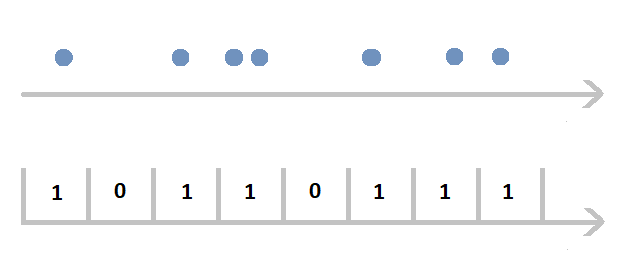
\includegraphics[scale=0.7]{Sp_t.png}
\end{figure} 

We model the variable $s_i(t)$ as a non-homogeneous Bernoulli process with expected value $\lambda (t)$, also referred to as \textit{spike rate}, that can be understood as the probability that the neuron will fire in the time bin $t$. Within the Bernoulli GLM framework, introduced in section \ref{Intro_GLM}, the spike rate is calculated from some linear predictor, $\eta_i(t)$ through a logit link function. 

\begin{equation}
\label{eq:prob}
\begin{split}
P(s_i(t)|\lambda_i(t)) =  Ber(\lambda_i(t)) = \lambda_i(t)^{s_i(t)}(1-\lambda_i(t))^{1-s_i(t)}, \\ \lambda_i(t) = h(\eta_i(t))= \frac{exp(\eta_i(t))}{1+exp(\eta_i(t))}.
\end{split}
\end{equation}

In our neural network model the linear predictor is a linear combination of the states of the neurons at the previous time step and a background noise, $b_i$. This is expressed as,

\begin{equation}
\label{eq:lin_pred}
    \eta_i(t) = \Big (\sum_{j=0}^{N}  w_{ji}(t)s_j(t-1) \Big) + b_i.
\end{equation}

Here $w_{ji}$ is a \textit{weight} between neuron $j$ and neuron $i$, and represents the strength of the connection between the two neurons. The contribution to the linear predictor for $\lambda_i(t)$ from neuron $j$ is $w_{ji}s_j(t-1)$. A positive value for $w_{ji}$ corresponds to an excitatory synaptic connection, whereas a negative weight represents an inhibitory one. A weight with value zero, means that there is no connection. Typically these weights are considered as stationary. However, as the aim is here to study the synaptic plasticity, the weights are let to vary with time. Therefore, we set $w_{ji} = w_{ji}(t)$. The connectivity of the whole network of neurons can thus be summarized by a time dependent $N \times N$ weight matrix, $W(t)$, which for three neurons would look like, 

\begin{equation*}
W(t) = 
\begin{pmatrix}
w_{11}(t) & w_{12}(t) & w_{13}(t)\\
w_{21}(t) & w_{22}(t) & w_{23}(t)\\
w_{31}(t) & w_{32}(t) & w_{33}(t)\\
\end{pmatrix}.
\end{equation*}

The weights $w_{ij}$ and the bias $b_i$ are then the regression coefficient $\bm {\beta}$ introduced in section \ref{sec:stats} for this network model. The parameters we aim to infer from the spike data.


%For the whole system of neurons, the probability for the state at time $t$ is,

%\begin{equation}
    %P(S_t|W_t) = \prod_{i,t} P(s_{it}|S_{t-1}, W_t).
%\end{equation}

 %where $\{t_1, t_2, ..., t_n\}$ is \ a sequence of equally spaced time steps in [0,T], where $t_{k}-t_{k-1} = t_1$.  To keep as much information as possible, it is preferable to set the time intervals so small that there is very low probability that the neuron will spike more than once in the intervals. Then, at time $t$ we have a collection of $N$ sequences

%\begin{equation}
    %S_{t} = \{\{s_{i,t_1}, ,...,s_{i,t-1},s_{it}\}\}_{i=0}^{N} \quad s_{i,t_k} \in {0,1}
%\end{equation}


\subsection{Inferring time varying weights}
The goal of this project is to learn the time varying weighs given the set of spiking values. As mentioned in chapter \ref{ch:theory} it is preferable to use a Bayesian approach, so one can include prior information. The prior will later be defined in terms of learning rules, but for this project it is set to be a restriction on how much a weight is allowed to vary from one time step to another. So, the prior distribution we will use is a gaussian distribution for each $w_{ji}(t)$ centered at $w_{ji}(t-1)$, each with standard deviation $\sigma$, namely

\begin{equation}
    P(W) = \frac{\exp(-\Gamma /2\sigma^2)}{\sqrt{2\pi \sigma^2}},
\end{equation}

where $W=\{W(t)\}_{t=1}^N$, and

\begin{equation}
    \Gamma = \sum_{j=0}^{N} \sum_{t=0}^{T-1} (w_{ji}(t+1)-w_{ji}(t))^2.
\end{equation}

Even though this is a simple prior to be used to test purposes, it is reasonable since we know that the true weights are correlated in time. 

Let $S(t) = \{s_i(t)\}_{i=1}^N$ be the collection of spike data for all the neurons at time $t$. As deduced from equation \ref{eq:prob} and \ref{eq:lin_pred}, all information about the spike rate of neuron $i$, $\lambda_i(t)$, is covered by the weights, the spike data in time step $t-1$ and the background rate $b_i$. Since the spike data and the background rate are considered as know, we can set

\begin{equation}
    P(s_i(t)|\lambda_i(t)) = P(s_i(t)|S(t-1),W(t), b_i) = P(s_i(t)|W(t)),
\end{equation}

which is the likelihood of $s_i(t)$ given some specified $W(t)$. The likelihood for all the spike data, $D=\{S(1), S(2)...,S(T)\}$ is then

\begin{equation}
\label{eq:lh}
    P(D|W) = \prod_{i,t} P(s_i(t)|W(t)),
\end{equation}

since the neurons are conditionally independent given the spike rate. Hence, we have the following expression for the posterior distribution for the weights

\begin{equation}
\label{Posterior}
        P(W|D) = \frac{P(D|W)\times P(W)}{P(D)} = \frac{\Big\{\prod_{i,t} P(s_{i}(t)|S(t-1), W(t))\Big\} \times \Big\{\frac{\exp(-\Gamma /2\sigma^2)}{\sqrt{2\pi \sigma^2}}\Big\}}{P(D)}, 
\end{equation}

where $P(D)$ is the marginal likelihood,

\begin{equation}
\label{eq:denominator}
        P(D) = \int \Big\{\prod_{i,t} P(s_{i}(t)|S(t-1), W(t))\Big\} \times \Big\{\frac{\exp(-\Gamma /2\sigma^2)}{\sqrt{2\pi \sigma^2}}\Big\} d{W}.
\end{equation}

Inference here will be performed by sampling the posterior distribution in equation \ref{Posterior} via the Metropolis Hastings algorithm described in section \ref{Metropolis}. For implementing this method one needs to evaluate the  ratio between the posterior for some suggested weights $W'$ and the current weights $W$. By taking this ratio and using equation \ref{Posterior} for the posterior, the marginal likelihood P(D) can be neglected. So computing $P(D)$, as in equation \ref{eq:denominator}, is unnecessary. Still one has to evaluate the model likelihood $P(D|W)$ which involves a product of probabilities over time, see equation \ref{eq:lh}. The product of factors less then one will decrease towards zero as the number of factors increases. Therefore, to avoid computer rounding to zero of the likelihood for a large number of time steps, it is preferable to use the log values for computations instead. The relevant value to compute in each iterations is then the following,

\begin{equation}
\label{eq:ratio}
\begin{split}
    \log \frac{\big \{ \prod_{i,t} P(s_{i}(t)|S(t-1), W(t)'\big \} \times \exp(-\Gamma' /2\sigma^2)}{\big \{ \prod_{i,t}  P(s_{i}(t)|S(t), W(t)) \big \} \times \exp(-\Gamma /2\sigma^2)} \\
    = \Big \{ \sum_{i,t} \log( P(s_{i}(t)|S(t-1), W(t)')) - \log( P(s_{i}(t)|S(t-1), W(t)) \Big \} -\Gamma' /2\sigma^2 +  \Gamma /2\sigma^2
\end{split}
\end{equation}

The parameter, $\sigma$, will be referred to at the \textit{prior standard deviation}. This can be adjusted to vary the dominance of the prior distribution. 


\section{Method for test cases}
\label{Method}

In this project three test cases were performed on a simple system consisting of two neurons, 1 and 2, and a synaptic weight, $w_{12}$ directed from neuron 1 to neuron 2.

\begin{figure}[h]
    \centering
    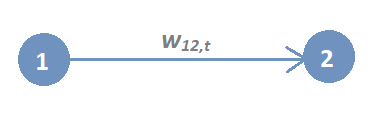
\includegraphics[scale=0.6]{Two_neurons_illustration.png}
\end{figure}

Neuron 1 has a constant probability for spiking, according to a background parameter $b_1$. Neuron 2 has spiking probability that depends on the spiking of $N_1$ in the previous time step through the linear predictor $b_2 + w_{21}(t) \cdot s_{1}(t-1)$. The actual spiking rate is related to the linear predictor through a logit link, as described in section \ref{sec:stats}. The distributions of the stochastic variables $s_{i}(t)$, representing the spiking in this system, are given by equation \ref{Eq:TestCase}.

\begin{equation}
\begin{split}
\label{Eq:TestCase}
    s_{1}(t) \sim \text{Ber}(\pi_{1}(t)) \hspace{3cm} \pi_{1}(t)= \frac{1}{1+e^{-b_1}} \\
    s_{2}(t) \sim \text{Ber}(\pi_{2}(t)) \hspace{1cm} \pi_{2}(t)= \frac{1}{1+e^{-(b_2 + w_{21}(t) \cdot s_{1}(t-1)}}
\end{split}
\end{equation}

Typical parameter values to be used in the test cases are 0.5 and 1 for b1, and -1 and 0 for b2. The value for the weight $w_{12}$ will be let to vary with time, but a typical size for it will be $w_{12}=0.7$. To get a better intuition it is useful to translate this to the corresponding firing rates. Table \ref{table:parameters} shows the resulting firing rates for the different parameter values


\begin{table}[!h]
\centering
\begin{tabular}{|c|c|c|c|}
	\hline
	Neuron & b & \pi_{s_{1}(t-1)=0} & \pi_{s_{1}(t-1)=1} \\
	\hline\hline
	1 & 0 & 0.5 & 0.5\\
	\hline
	1 & 0.5 & 0.62 & 0.62\\
	\hline
	2 & -1  & 0.27 & 0.43\\
	\hline
	2 & 0  & 0.5 & 0.77\\
	\hline
\end{tabular}
\caption{Background parameter and corresponding spiking rates for neuron 1 and neuron 2}
\label{table:parameters}
\end{table}

The purpose of all the test cases was to infer the underlying weights given the spike train data. Normalized root mean square error (rnMSE) was used to measure the performance of our method in all tests cases. This was calculated according to the following equation,

\begin{equation}
    rnMSE = \sqrt{\frac{\sum_t(w_{12}(t)^I-w_{12}(t))^2}{\sum_t w_{12}(t)^2}},
\end{equation}

where $w_{12}(t)^I$  are the inferred weights and $w_{12}(t)$ are the generative weights.

\subsection{CASE 1: Inferring a constant weight with Newton method}
\label{sec:CASE1}

In case 1 the series of Bernoulli variables $\{s_{1}(t)\}_{t=1}^T$ and $\{s_{2}(t)\}_{t=1}^T$ were drawn according to equations \ref{Eq:TestCase}, with constant weight $w_{21}(t) = w_{21} = 0.7$ and $T=1000$. The score and Fisher value for this situation is 

\begin{equation}
\begin{split}
    score(w_{12}) = \sum_{t=2}^{T} s_{1}(t-1) (s_{2}(t)-\pi_{2}(t)), \\
    H(w_{12}) = \sum_{t=2}^T s_{1}(t-1)^2 \pi(t)(1-\pi(t)) = \sum_{t=1}^T s_{1}(t-1) \pi(t)(1-\pi(t)).
\end{split}
\end{equation}

The last equivalence is valid since $s_{1}(t)$ only can take values 1 or 0. 

An initial guess was set to $w_{12}^{(0)} = 2$. Newton iterations, as given by equation \ref{eq:Newton}, were performed until convergence.\\ 

\subsection{CASE 2: Inferring dynamic weights with Metropolis-Hastings}
\label{sec:CASE2}
Now the weights were let to vary, and the aim was to infer the vector of weights ${\bf w_{12}}$ in time T, which was set equal to 10. In the first time step, there is no "previous step" that can be used to evaluate the spike rate of neuron 2. Therefore, in this time step the only thing happening is generating the variable $s_{1}(1)$. This means that there are 9 weights to infer, corresponding to $t=2,...,10$. From $t=2$, spikes for both neurons are generated, where the spike rate for neuron 2 is computed according to the value of the linear predictor. 

Before simulating spiking of the two neurons, the generative weight trajectory was specified. The weight at $t=2$ was set to 0.7, and the remaining weights were drawn as

\begin{equation}
    w(t) = w(t) + |n(0,0.001)|,
\end{equation}

where $|n(0,0.001)|$ is the absolute value of a normal distributed variable with zero mean and variance equal to $0.001$. The absolute value is used so that the weight trajectory imitates a connection that strengthens over time. Figure \ref{fig:Generative} shows an example of how a typical generative weight trajectory for this test case looks like. 

\begin{figure}
\caption{Example generative weight trajectory in case 2}
\label{fig:Generative}
    \centering
    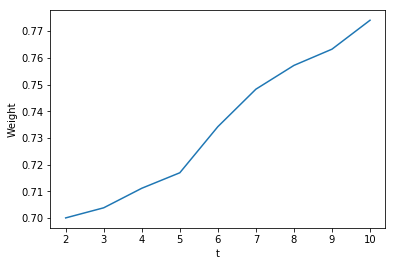
\includegraphics[scale=0.8]{fig/UL.png}
\end{figure}


In reality the number of time steps is much larger, and changing much slower. However, few time steps is used in this test case for simplicity and shorter running time. Therefore, the plasticity is set high so that it is possible to investigate whether the algorithm can infer time varying weights and not only approximates to a constant value. 

Spike trains for the two neurons were drawn according to equation \ref{Eq:TestCase}, this time using the generated time varying weights. These spike trains were drawn various number of times for the same weight trajectory, for comparing the goodness of the algorithm for different amounts of data. In other words, for one weight trajectory $\{w_{12,t}\}_{t=1}^T$ we simulated spike trains
$\{\{s_{1}(t)_i\}_{t=1}^T\}_{i=1}^I$ and $\{\{s_{2}(t)_i\}_{t=1}^T\}_{i=1}^I$ with $I \in \{1,10,100,1000,10000 \}$.

To infer the weights from the data, the Metropolis-Hastings algorithm was used. In the algorithm the logarithm of the rejection ratio given by \ref{eq:ratio} needs to be computed in every iteration. For this two neuron system, the log-rejection ratio reads:

\begin{equation}
    \log ( \alpha) = l({\bf w_{12}}') - l({\bf w_{12}}) - \Gamma({\bf w_{12}}')/2\sigma^2 + \Gamma({\bf w_{12}})/2\sigma^2,
\end{equation} 

with

\begin{equation}
\begin{split}
    l({\bf w_{12}}) = \sum_i \sum_t s_{2,i}(t)(b_2 + w_{12}(t)*s_{1,i}(t-1)) - \log(1 + \exp(b_2 + w_{12}(t) * s_{1,i}(t-1))), \\
    \Gamma({\bf w_{12}}) = \sum_{t=2}^T (w_{12}(t) - w_ {12}(t-1))^2.
\end{split}
\end{equation}

In this case the prior variance was equal to $ 0.0001$. The proposal distribution used was a multivariate normal distribution with mean vector equal to the weight trajectory from the last iteration, variances equal to $0.0001$ and zero covariances. 
The Metropolis-Hastings procedure for this case is summarized in algorithm \ref{alg:M-H}.

\begin{algorithm}
\caption{}\label{alg:M-H}
\begin{algorithmic}
\State Create empty list $[]$ for weight sample
\State Set start guess ${\bf w_{12}} = {\bf w_{12}}^{(guess)}$
\For {$iteration=1,2,\ldots$}
\State Draw ${\bf w_{12}}'$ from proposal distribution
\State Compute $\log(\alpha)$
\State Compute $\alpha = \exp(\log(\alpha))$
\If {$\alpha > 1$}
\State ${\bf w_{12}} = {\bf w_{12}}'$
\Else 
\If {random.uniform(0,1) $<\alpha$}
\State ${\bf w_{12}} = {\bf w_{12}}'$
\EndIf
\EndIf
\State Add ${\bf w_{12}}$ to sample list
\EndFor
\end{algorithmic}
\end{algorithm}

Two variants of this procedure was performed. First, the initial guess was set equal to the generative weights. This gives insight into how much the procedure would drift away from the generative connections. In reality the true weights are not known. Therefore, it is also relevant to check whether the generative weights can be inferred when starting somewhere else. So in the second variant the initial guess was a random walk around 1. 

\subsection{CASE 3: Weights generated by learning rule}
In reality it is not possible to perform multiple spiking replicates for the same weight trajectory. If the synaptic connections are changing according to learning rules, as presented in section \ref{sec:LR}, the weight updates are dependent on the spiking as time goes by. Since the spiking is a random process, it cannot be reproduced properly. Therefore, we have to rely on only one spike train per neuron, for one weight trajectory. However, for the system we are tailoring this method to we may expect long time series, weights changing on a longer time scale than the spiking one and strongly correlated. We then aim at leveraging these properties for inferring the weights. 

So in this test case weights and the spikes were generated simultaneously, by means of the STDP learning rule, given by equation \ref{eq:STDP}. The parameter values used for the learning rule were the same as the ones suggested in \cite{Song}, namely $\tau_{\pm} = 20 ms$, $A_+ = 0.005$ and $A_- = 1.05 \times A_+$. The learning rule with these parameters is illustrated in figure \ref{fig:LR}.

\begin{figure}[hbt!]
\caption{STDP learning rule}
\label{fig:LR}
    \centering
    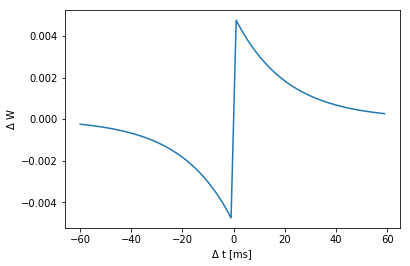
\includegraphics[scale=0.8]{fig/Learning_rule2.png}
\end{figure}

This time $T$ and the spiking rates are set to illustrate realistic time relations. In \cite{Linderman} the authors use a baseline firing rate with mean 20Hz. To roughly have the same firing level the model was set to have 40 time stamps for representing one second, and the firing rate of the two neurons around one half. 

First the procedure in algorithm \ref{alg:M-H} was performed with 10 seconds (T=400 time stamps). The weight trajectory drawn for this is plotted in figure \ref{fig:w_STDP}. 


\begin{figure}[hbt!]
\caption{Generative weights drawn according to the STDP rule and the generated spikes}
\label{fig:w_STDP}
    \centering
    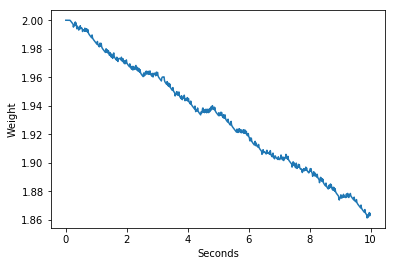
\includegraphics[scale=0.8]{fig/LR_underllying.png}
\end{figure}

An easy way to simplify the problem by utilizing the time correlations is to specify equally sized time windows and assume that the weight is constant within each window. Since we have restricted the degrees of freedom this can only give a rough estimate of the weights. However, for later work we are going to characterize the parameters of the learning rule itself rather than the weights. So since the number of parameters in the learning rule is significantly less than the number of weights, any precise and detailed inference of each weight is actually not needed. Therefore, it is useful to investigate whether strict constrains makes it possible to capture some learning trends with only one spike trajectory.


%\section{Precalculations}
%\label{Precalc}

%\begin{itemize}
    %\item The aim here is to calculate how well I expect my tests to work. Can use hypothesis testing on bernoulli GLM 
    %\item Say something about how many time points ect that is needed to be able to detect a change of the weights
%\end{itemize}

%\begin{wraptable}{r}{4cm}
%\begin{center}
 %\begin{tabular}{||c c c ||} 
 %\hline
% n & Lower & Upper \\ [0.5ex] 
% \hline\hline
% 10 & 0.5 & 1 \\ 
% \hline
 %100 & 0.7 & 0.84 \\
 %\hline
 %1000 & 0.748 & 0.792 \\
 %\hline
 %10000 & 0.7631 & 0.7769 \\ [1ex] 
 %\hline
%\end{tabular}
%\end{center}
%\end{wraptable}

%\begin{figure}[h]
   % \centering
    %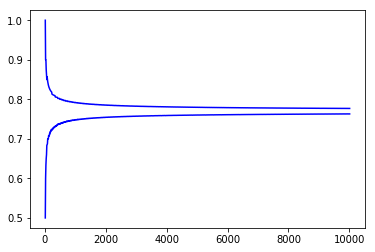
\includegraphics[scale=0.7]{Conf_intervals.png}
%\end{figure}

%It is practical to have some understanding of how precisely the weights can be inferred from the spike data. When performing $n$ repeated trials of a Bernoulli process with success rate $\pi$, the sum successes comes from a binomial distribution, with parameters $n$ and $\pi$. For some success count, $n_{success}$, the parameter $\pi$ can be estimated as $\frac{n_{success}}{n}$. How good this estimate is depends on the number of trials, $n$. Figure ?? and table ?? presents the endpoints of range that contains 90\% of the distribution, for different values of n (scaled by one over n). 
%===================================== CHAP 5 =================================

\chapter{Results}
\label{ch:results}

The results from performing the test cases described in section \ref{Method} are presented in this chapter. Section \ref{sec:CASE1_r}, \ref{sec:CASE2_r} and \ref{sec:CASE3_r}, gives the results from test case 1, 2 and 3 respectively. Plots of errors and visualizations of the estimates are given. The focus in this project has been to investigate how well the methods for inferring weight perform, and not to study any actual weights. Therefore, any detailed description of what the inferred weights values are is not included.

\section{CASE 1}
\label{sec:CASE1_r}
50 iterations Newton iterations for a constant true weight, $w_{21} = 0.7$, for $T=1000$ and initial guess $w_{12}^{(0)} = 2$ was performed according to the description in section \ref{sec:CASE1}. The estimated weigh after the last iteration was $w_{21}^{(50)}=0.679$. The left plot in figure \ref{fig:Newton} illustrates the likelihood function, and the points for the initial guess, and the estimated weight after 1, 2, 3 and 50 iterations. The right plot shows the estimated weigh at every iteration.

%The learning was on purpose set slower, in order to give a better visual representation. 


\begin{figure}[hbt!]
\caption{(Left) Log-likelihood with starting point, 1st, 2nd, 3rd and 50th iteration marked. (Right) Estimated weight for each iteration.}
\label{fig:Newton}
    \centering
    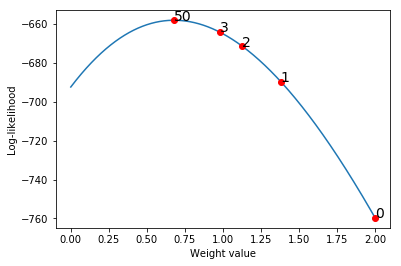
\includegraphics[scale=0.40]{Step_1.png}
    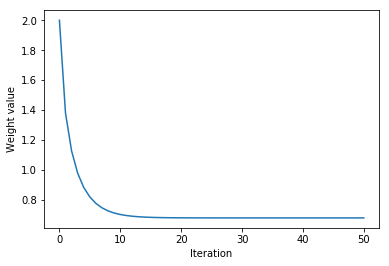
\includegraphics[scale=0.40]{fig/Step_1_it.png}
\end{figure}

One can conclude that the algorithm converges by visual inspection of the plots. Also, the estimated weight in the five last iterations are equal up to seven decimals. To arrive at two decimals precision it took 18 iterations. However, the inferred weight and the true weight differ by $w_{21} - w_{21}^{(50)} = 0.021$. This difference is not due to any failure of the algorithm to find the maximum likelihood, but rather due to the fact that for a finite data sample the actual maximum likelihood value in the data might differ from the underlying parameter that generated them. This will improve as the size of the data set increases. To illustrate this point, the algorithm was run 1000 times each for $T \in \{ 100,1000,10000\}$. Histograms for the maximum likelihood estimates is shown in figure \ref{fig:ML_hist}. By looking at the axes it is clear that in all cases the estimates are centered around the true value, but for a bigger sample the variance in the estimates are smaller. 

\begin{figure}[hbt!]
    \centering
    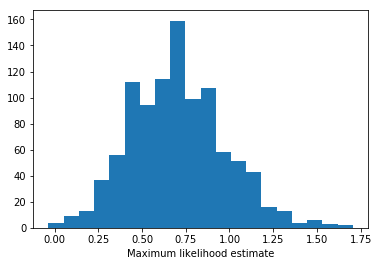
\includegraphics[scale = 0.40]{fig/ML_100.png}
    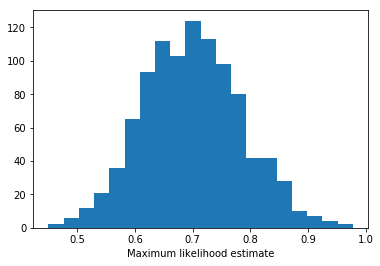
\includegraphics[scale = 0.40]{fig/ML_1000.png}
    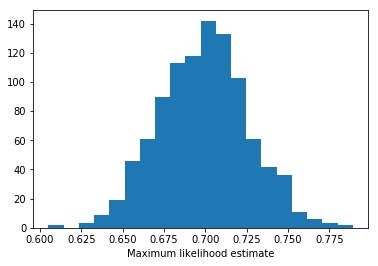
\includegraphics[scale = 0.40]{fig/ML_10000.png}
    \caption{Histograms of estimated weighs from 1000 replicates with 100 (top left), 1000 (top right) and 10000 (bottom) time steps}
    \label{fig:ML_hist}
\end{figure}

\section{CASE 2}
\label{sec:CASE2_r}
The procedure described in section \ref{sec:CASE2}, and summarized in algorithm \ref{alg:M-H} was performed with 3000 iterations, for various number of spike trains, $ \{1,10,100,1000,10000 \}$. Firstly, the initial guess was set equal to the true weights, namely $\bf w_{12}^{(0)} = \bf w_{12}$. This gives a starting error of zero. Figure \ref{fig:Case2_1} shows an example of normalized root mean squared errors over iterations for the different number of trials. Here the generative weight trajectory, as exemplified in figure \ref{fig:Generative} was the same for all the instances, and the initial guess was set to be the true weights. 


\begin{figure}[hbt!]
\caption{Normalized root MSE over iterations for various number of trials. One example of the method in case 2 when starting from the correct weights}
\label{fig:Case2_1}
    \centering
    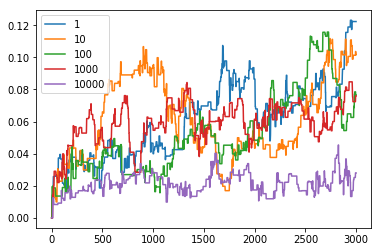
\includegraphics[scale=0.6]{MSE3.png}
\end{figure}

This shows that for the lower number of trials the estimation jumps around, whereas for 10000 trials it is more stable.

This procedure was repeated 100 times for each number of trials. The underlying weights were now drawn new for each replicate. Figure \ref{fig:case2_avg} shows the mean of the rnMSE values at each iteration, with variance bars around it. 

\begin{figure}[hbt!]
\caption{Average rnMSE with variance bars of 100 replicates for each number of trials. Initial guess set to the true weights.}
\label{fig:case2_avg}
    \centering
    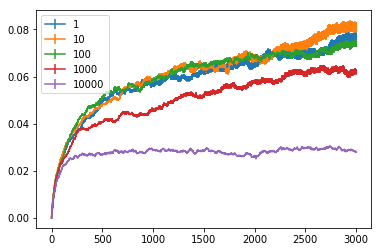
\includegraphics[scale=0.6]{Mean_plot_std.png}
\end{figure}

%\begin{figure}[hbt!]
    %\centering
    %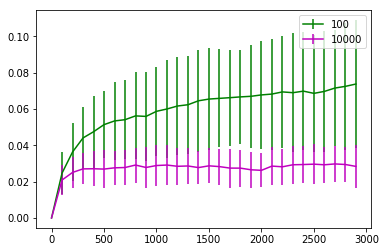
\includegraphics[scale=0.8]{Std_every100.png}
%\end{figure}


Next, the initial guess for the iterations is set to be a random walk around 1. Figure \ref{fig:MSE2} shows the corresponding mean rnMSE of 100 replicates for each number of trials, with variance bars. 

%\begin{figure}[hbt!]
    %\centering
    %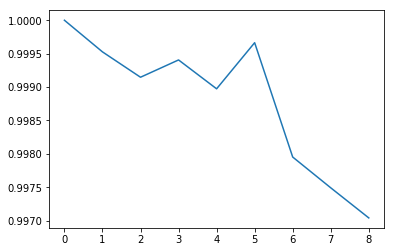
\includegraphics[scale=0.8]{Start_it_1000.png}
%\end{figure}


\begin{figure}[hbt!]
\caption{Average rnMSE with variance bars of 100 replicates for each number of trials. Initial guess set to random walk around 1}
\label{fig:MSE2}
    \centering
    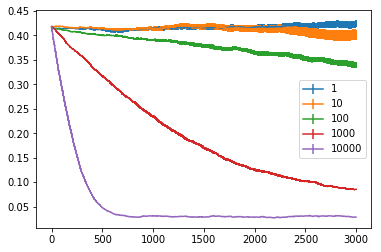
\includegraphics[scale=0.6]{MSE_starting_away.png}
\end{figure}

As clear from the plots, the relaxation time for the learning is dependent on the number of trials. For initial guess equal to the generative weights, saturation happens after around 300 iterations for 10000 trials, and around 2500 iterations for 1000 trials. For less number of trials the solution is still moving away from the solution after 3000 iterations. Figure \ref{fig:MSE2} show that also for 100 trials there is a slow movement in the correct direction. The figures also show that the solution is more stable for the higher number of trials, since the variance bars are thinner.  

To visualize what is happening during the course of the iterations figure \ref{fig:trajectories} displays the how the last accepted weight trajectory to the sample after 100,200,300,400,500 and 1000 iterations looks like, for initial guess a random walk around 1 and 10000 trials. 

Figure \ref{fig:trajectories} shows that the weight trajectory shifts rigidly across iterations towards the generative value, and eventually ends up relatively close to the true weights. This is enforced by the prior distribution, which demands a continuity in time. 

\begin{figure}[P]
\caption{Plots of the true weights (blue), the initial guess (orange), and the inferred weights after 100, 200, 300, 400, 500 and 1000 iterations (green)}
\label{fig:trajectories}
    \centering
    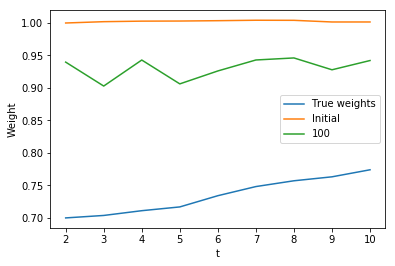
\includegraphics[scale=0.4]{fig/10000_100.png}
    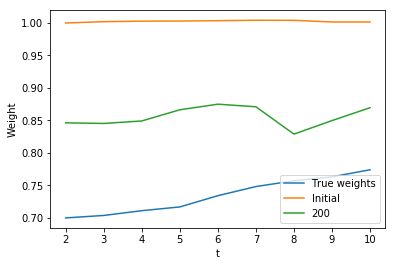
\includegraphics[scale = 0.4]{fig/10000_200.png}\\
    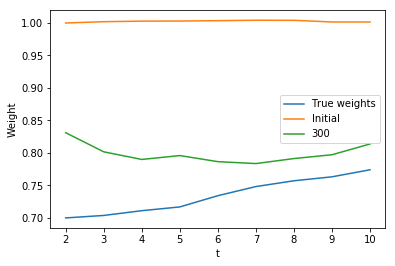
\includegraphics[scale = 0.4]{fig/10000_300.png}
    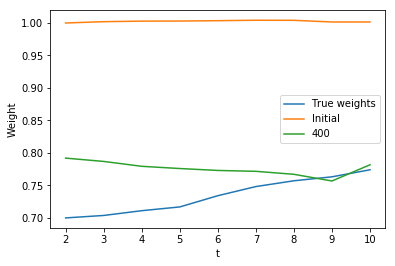
\includegraphics[scale = 0.4]{fig/10000_400.png}\\
    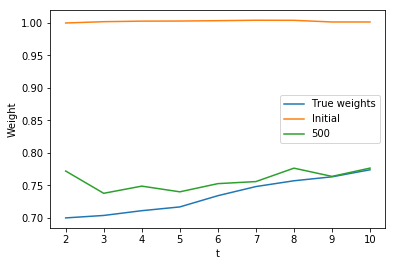
\includegraphics[scale = 0.4]{fig/10000_500.png}
    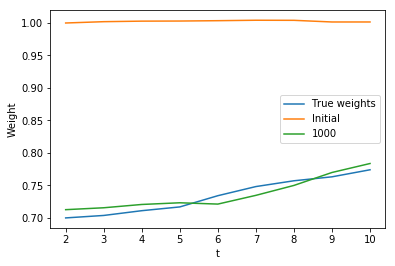
\includegraphics[scale = 0.4]{fig/10000_1000.png}
\end{figure}

It was also investigated what happens during the iterations for a lower number of trials. For exemplification, with 10 trials various values for the prior variance was tried to see if the results could be improved. All variants gave fluctuating error over iterations, except when the prior was set so strict that no steps were accepted. Figure \ref{fig:10st} illustrates the weight trajectory after 10000 iterations for prior variances in $\{ 0.1, 0.01, 0.001, 0.0001, 0.00001\}$. 10000 iterations was chosen to be sure that if any convergence took place, this would be shown. 

\begin{figure}[P]
\caption{Plots of the true weights (blue), the initial guess (orange), and the inferred weights after 10000 iterations with 10 spike trains, and a prior variance of 0.1, 0.01, 0.001, 0.0001 and 0.00001}
\label{fig:10st}
    \centering
    \includegraphics[scale=0.4]{{10st_0.1prior}.png}
    \includegraphics[scale = 0.4]{{10st_0.01prior}.png}\\
    \includegraphics[scale = 0.4]{{10st_0.001prior}.png}
    \includegraphics[scale = 0.4]{{10st_0.0001prior}.png}\\
    \includegraphics[scale = 0.4]{{10st_0.00001prior}.png}
\end{figure}

As seen the starting trajectory used here is quite flat. One could think that this could stop the trajectory from moving away from its starting position, since it is already too good in terms of the prior. Therefore it was also tried a much more variate starting point, and a strict prior variance of 0.00001, to see the result then. The weight after 10000 iterations for this variant is shown in figure \ref{fig:10st2}.

\begin{figure}
    \centering
    \includegraphics[scale=0.6]{{10st_0.00001prior_1starting}.png}
    \caption{Plots of the true weights (blue), the initial guess (orange), and the inferred weights after 10000 iterations with 10 spike trains, and a prior variance of 0.00001. Initial weight trajectory for the iterations were drawn with }
    \label{fig:10st2}
\end{figure}


\section{CASE 3}
\label{sec:CASE3_r}
First the variant where the weight for all time steps are drawn individually were performed. This was tried with various values for the variance in the prior and proposal distribution. For a low value of the prior variance compared to the proposal variance, no new weight trajectories were accepted in the algorithm, so the estimation just stays where it starts. If the relative variance is large enough for weight trajectories to be accepted, it does not move towards the correct solution, and the error increases with iteration. One example of the true, initial and inferred weights after 3000 iterations is shown in figure \ref{fig:400_weights}. 


\begin{figure}
    \caption{True weights (orange), initial guess (green) and inferred weights (blue) after 3000 iterations}
    \label{fig:400_weights}
    \centering
    \includegraphics[scale=0.6]{fig/{Result_0.08}.png}
\end{figure}


Next, the same procedure was performed with dividing the time line into windows, and assuming constant weights within the windows. The initial guess was set to a random walk around 1. The result for dividing 300 seconds into 10 windows, and performing 3000 iterations is shown in figure \ref{fig:10bins}, with prior and proposal variance equal to 0.01, 0.005 and 0.0005.


\begin{figure}[hbt!]
\caption{True weights (orange), initial guess (green) and inferred weights (blue) for 10 bins and 3000 iterations. The prior and proposal distribution was 0.01 (top left), 0.005 (top right) and 0.0005 (bottom)}
\label{fig:10bins}
    \centering
    \includegraphics[scale=0.45]{fig/{10bins_0.01_0.01_s}.png}
    \includegraphics[scale=0.45]{fig/{10bins_0.005_0.005_s}.png}\\
    \includegraphics[scale=0.45]{fig/{10bins_0.0005_0.0005}.png}
\end{figure}

Figure \ref{fig:10bins} shows that $0.01$ and $0.005$ gives a reasonable result, whereas $0.0005$ forces a time continuity that is too strict to properly capture the dynamics.

This was done for 1, 5, 10 and 20 number of windows, with 30 replicates for each. The mean of the rnMSE with variance bars for these are presented in figure \ref{fig:MSE_bins}. Here the prior and proposal variance used was 0.005, which was chosen as it gave reasonable results. 

\begin{figure}[hbt!]
\caption{}
\label{fig:MSE_bins}
    \centering
    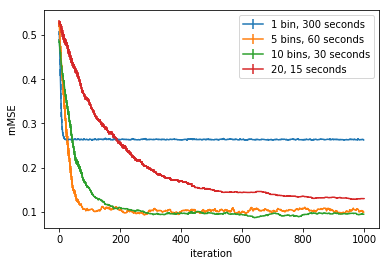
\includegraphics[scale=0.6]{fig/MSE_bins.png}
\end{figure}


It is clear from figure \ref{fig:MSE_bins} that there is a trade-off between the constraint imposed by the time windows and the ability to update towards likelier parameters. With 10 windows the number of weights to infer is almost the same as in test case 2, where there was 9. However, it is interesting to note saturation is reached faster. The value of the rnMSE is bigger than in case 2. This is reasonable, as we set a constant weight in each window when the true weight is varying over the window. 

\begin{figure}[hbt!]
\caption{Plot of average rnMSE of 20 replicates with 10 windows for prior variances equal to 1, 0.1, 0.02 and 0.005}
\label{fig:prior_variance}
    \centering
    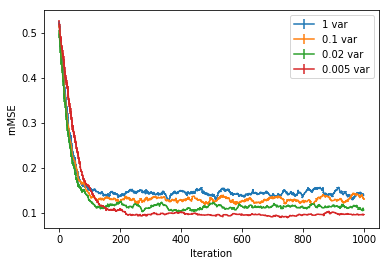
\includegraphics[scale=0.6]{fig/Prior_variance_plot.png}
\end{figure}


\cleardoublepage
%===================================== CHAP 6 =================================

\chapter{Discussion and conclusion}
\label{ch:6}

To wrap up the project work, this chapter presents some summary and remarks. Section \ref{sec:review} provides discussion and additional notes of the results. For my master thesis the goal is to expand this work. Some of the ideas for further work is presented in section \ref{sec:FW}. Section \ref{sec:conclusion} presents some summarizing statements and the main conclusions.  

\section{Reviewing the results}
\label{sec:review}
\subsection{Summary}
Through the methods described in section \ref{Method} the strength one time-varying synaptic connection was investigated. In chapter \ref{ch:results} the results from performing the three test cases were presented. From test case 1 with a static weight, it was shown that Newton iterations was a sufficient method to learn the weight. It was also demonstrated how variate the maximum likelihood value of the weight was for different sizes of the data set. In test case 2 is was investigated how a Bayesian framework and Metropolis-Hastings inference worked to infer dynamical weights for varying amounts of data, in a simple case with weights for nine time steps. Section \ref{sec:CASE2_r} presents plots of how the error develops over iterations for the different number of spike trains. It was also shown the movement of the weight trajectory through the iterations for the case with 10000 spike trains, and the result of 10 spike trains with varying prior variance. Finally, in case 3 the intention was to study a situation that was closer to how the real data is expected to be. The generative weight trajectory was longer and based on the additive STDP rule, and there was one spike train only. It was shown that the method did not work when trying to infer a weight for every time step. The method was then investigated with constraining the weights to be constant within some equally sized windows. Different prior values and different length of the windows were tried and compared. The performance of the different versions are illustrated in figures \ref{fig:10bins} and \ref{fig:MSE_bins}. 

\subsection{Discussion} 

One of the main findings in the results is that, provided enough data, it is possible to infer the strength of a time varying synaptic connection from spike train data. It is clear from figure 5.3, 5.4, 5.5 and 5.6 that with 10000 spike trains for one generative weight trajectory, the method is able to infer each of the weights well enough to characterize the plasticity, that was an weight increase from about 0.7 to 0.8 for those cases. Figure 5.10 and 5.11 illustrates that with a long and slowly varying weight trajectory, trends in the weight dynamics can be captured with only one spike train provided that we have proper constraints. This variant gives good indications that learning trends will also be possible to capture in real data. 

Another important observation is that, with the little amount of information contained in the prior, few data points gave bad results. A single weight can for example not be inferred with 1 or 10 data points, with the smoothness prior. This was however not surprising. As indicated in the histograms from case 1, even with 100 data points for a single weight it is not unlikely that the maximum likelihood value for the weight as given by the data is above 0.9 or below 0.5, even though the data was generated with a weight value of 0.7. Therefore, one can not expect to for example detect a weight change from 0.7 to 0.8 from only 100 data points. For a smoothness prior, the best we can hope for is that it stabilizes around the mean weight.

Another problem with the method is that since all weights are drawn independently but simultaneously, the probability of drawing a weight trajectory that is considerably better than the previously accepted one gets very little when the weight trajectory is large. By considerably better we mean that a great proportion of the weights are drawn closer to the correct trajectory. Define success as the event that a weight is drawn to a better position than in the previous iteration, giving a success rate of 0.5. Then, we can consider drawing the whole trajectory as one binomial experiment. Then, for the case of 400 time steps, the probability of at least 225 successes is less than one percent. This is the problem in the first plot of case 3.  

It is also interesting to say something about the differences with the framework in this project compared to \cite{Linderman}. Since the method for inference is not the same, the results are not directly comparable. However, so far using a Bernoulli GLM compared to Poisson haven't shown to be problematic...

\section{Further work}
\label{sec:FW}

Even though the findings in this work gives insight for studying neural activity with dynamical connectivity, there was done some considerable simplifications. Therefore, before integrating it with real data, some changes will be made. In this project only activity one time step back in time for the presynaptic neuron was considered to calculate the rate of the postsynaptic neuron. This was not problematic for the inference here, as also the spike activity was simulated this way. For real data however, it is likely that also activity further back in time will have an effect, although the impact probably will decrease with a bigger time lag. Also, previous spiking of the neuron itself, not only of connected neurons will be relevant to consider. 

One main goal later will be to characterize the learning rule from the spike data, rather than the weight trajectory. The assumption that the connections change according to specified learning rules also provides additional information, that can be integrated in the prior. The particle MCMC method, as used in \cite{Linderman}, will be implemented. This will make it possible to infer a longer weight trajectory, as one weight will be considered at the time, although the weight trajectory itself is not the goal. 


\section{Conclusion}
\label{sec:conclusion}

The aim in this work was to develop a method for studying synaptic plasticity by using statistical tools. The motivation for this research topic was that synaptic plasticity is an important function for memory, so knowledge in this field can be a useful contribution to studying memory related diseases. 

In this project a system of two neurons and a single synapse was considered. The activity of the postsynaptic neuron was modeled by a Bernoulli Generalized Linear Model, with a time-varying spike rate that was related to previous activity of the presynaptic neuron through a linear predictor and a logit link function. The connection strength was represented by a time dependent weight. A Bayesian approach with a smoothness prior was taken, and the Metropolis-Hastings algorithm was implemented for inferring the weight trajectory. 

It was shown that provided enough spike data, the dynamical weights could be inferred with this method. This was demonstrated both by using multiple trials of data for a short weight trajectory, and by using a single spike train for a long weight trajectory with a strict constraint on the weights. As expected, with little data, it did not work well. To avoid a solution that jumps around, the prior has to be strict for little data. A strict smoothness prior results in a straight line that cannot learn any weight dynamics. Findings in case 3 suggest that if the weights are changing slowly, and recordings are made for a long time, trends in weight dynamics can be captured with only one spike train, providing enough constraints are set. This is a good indication that it can be possible to characterize the learning rules in real data. 



%\begin{itemize}
    %\item Short summary of the things that has been done in the project; Neurons form connections to each other, and these connections can vary with time. Various learning rules are hypothesized to govern these dynamics. The strength of connections is reflected by the spiking of neurons. Aim to develop a model to infer time varying connectivity based on spike train data. Spiking is modeled with Bernoulli GLMs. Metropolis-Hastings with smoothness prior used for inference. The method showed to work for enough data material. And as expected it did not work well for little data material per inferred weight. To avoid a solution that jumps around, the prior has to be strict for little data. A strict smoothness prior results in a straight line that cannot learn any weight dynamics. Findings in case 3 suggest that if the weights are changing slowly, and recordings are made for a long time, trends in weight dynamics can be captured with only one spike train.
    %\item The next goal is to infer parameters for the learning rules, rather than the weights. Also, particle MCMC will be used. This includes using the learning rules for the prior... 
%\end{itemize}



\cleardoublepage

%% PART 4
\pagestyle{fancy}
\fancyhf{}
\renewcommand{\chaptermark}[1]{\markboth{\chaptername\ \thechapter.\ #1}{}}
\renewcommand{\sectionmark}[1]{\markright{\thesection\ #1}}
\renewcommand{\headrulewidth}{0.1ex}
\renewcommand{\footrulewidth}{0.1ex}
\fancyfoot[LE,RO]{\thepage}
\fancypagestyle{plain}{\fancyhf{}\fancyfoot[LE,RO]{\thepage}\renewcommand{\headrulewidth}{0ex}}

\addcontentsline{toc}{chapter}{Bibliography}

\bibliographystyle{elsarticle-harv}
\bibliography{mylib}

\cleardoublepage	%% Edit your references in "mylib.bib"
\section*{\begin{center}{\Huge Appendix}\end{center}}
\addcontentsline{toc}{chapter}{Appendix}
$\\[0.5cm]$

\noindent Write your appendix here...		%% Optional

\end{document}